\documentclass[a4paper,11pt]{article}

% Packages
\usepackage{graphicx}
\usepackage{amsmath}
\usepackage{geometry}
\usepackage{fancyhdr}
\usepackage{setspace}
\usepackage{float}
\usepackage{titlesec}  % For title formatting
\geometry{margin=1in}
\usepackage{caption}
\usepackage{subcaption}
\usepackage{booktabs}
\usepackage{multicol}
\usepackage{wrapfig}
\geometry{left=0.8in, right=0.8in, top=1.2in, bottom=1.2in}
\setstretch{0.95}

% Header and Footer
\pagestyle{fancy}
\fancyhf{}
\fancyhead[L]{Challenge 1}
\fancyhead[R]{\thepage}

% Title Formatting
\titleformat{\section}{\normalfont\Large\bfseries}{\thesection}{1em}{}

% Cover Page
\title{
    \vspace{2cm} % Adjust vertical space
    
\includegraphics[width=0.55\textwidth]{Logo_Polimi.png} \\ % Add your logo here (change "logo.png" to the actual filename)
    \vspace{1cm} % Adjust vertical space after the logo
    \textbf{\Huge Challenge 2} \\
    \vspace{1cm} % Adjust vertical space
    \large Advanced Algorithms and Parallel Programming \\
    \vspace{0.5cm} % Adjust vertical space
    \large \date{\today}
}

\author{Camilo José Sinning López, Oliver Mosgaard Stege\\ \& Raul Eduardo Vergara Lacouture}


\begin{document}

% Title Page
\maketitle
\thispagestyle{empty}
\newpage

% Table of Contents
% Start page numbering from the Table of Contents
\setcounter{page}{1}  % Start counting from 1
% \tableofcontents
% \newpage


\section{Experimental Setup}

The program implements a parallel Sudoku solver using OpenMP. The algorithm recursively explores all possible solutions to a given Sudoku puzzle by assigning numbers to unfilled cells, ensuring no conflicts in rows, columns, or subgrids.

\subsection{Hardware and software}

All experiments were conducted on a laptop with the following processor details:

\begin{itemize}
    \item \textbf{Model:} AMD Ryzen 5 7520U with Radeon Graphics
    \item \textbf{Base Clock:} 2.8 GHz
    \item \textbf{Max Boost Clock:} Up to 4.3 GHz
    \item \textbf{Cores:} 4
    \item \textbf{Threads:} 8
\end{itemize}

\subsection{Algorithm parameters}

\begin{itemize}
    \item Grid Size: Dimension of the Sudoku puzzle (e.g., 9x9).
    \item Block Size: Size of subgrids (e.g., 3x3 for standard Sudoku).
    \item Max Depth: Specifies the depth for task creation in the parallel recursion.
    \item Threads: Maximum number of threads to use in the parallel algorithm.
    \item sudoku: The Sudoku puzzle to solve.
\end{itemize}

\subsection{Executions}

\subsubsection{Fixed depth}

The first set of experiments was conducted with a fixed max\_depth of 3. For each thread count, 3 samples were collected for 9x9 and 25x25 Sudoku puzzles.

\subsubsection{Variable depth}
The second set of experiments was conducted with a variable max\_depth. For thread counts ranging from 1 to 12, experiments were conducted for each max\_depth value in {3, 5, 7, 9}. Three samples were collected for each configuration.


\section{Performance Measurements}

Summarized results are saved in a CSV file with columns:

\begin{enumerate}
    \item Execution time.
    \item Grid size.
    \item Block size.
    \item Number of threads.
    \item Number of solutions.
    \item Max depth.
\end{enumerate}

Sample output: The program outputs the timing and results to the console and appends them to the times.csv file.

\section{Results}

The following results were taken from times.csv file, and only the threads available in the machine were used for to create the plots since more threads would not be beneficial.

\subsection{Fixed depth}

\begin{figure}[H]
    \centering
    \begin{subfigure}[b]{0.35\textwidth}
        \centering
        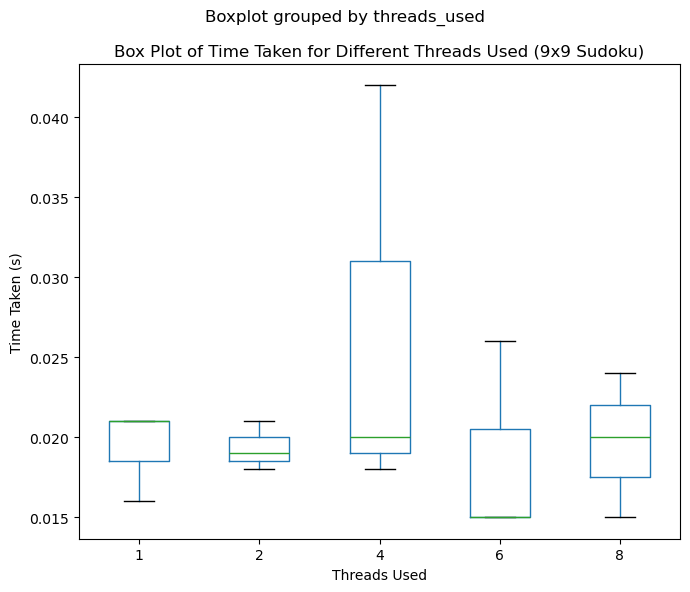
\includegraphics[width=\textwidth]{9x9_fixed_depth.png}
        \caption{Execution time for 9x9 Sudoku puzzles with fixed depth.}
    \end{subfigure}
    \hfill
    \begin{subfigure}[b]{0.35\textwidth}
        \centering
        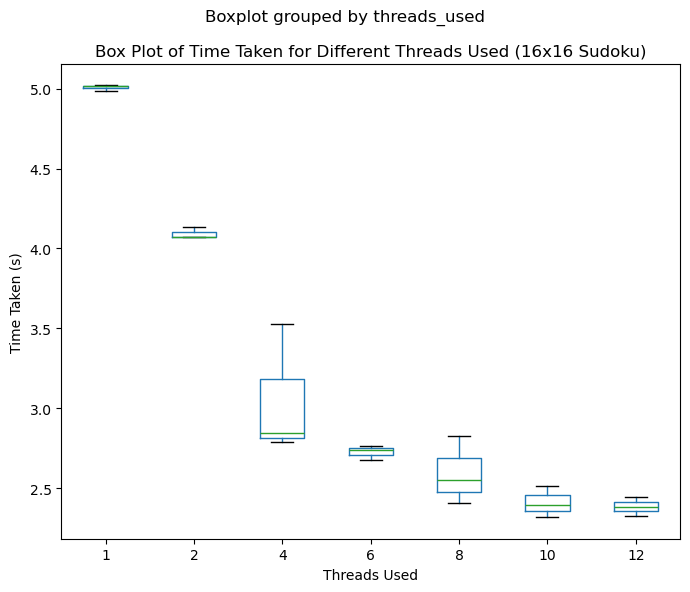
\includegraphics[width=\textwidth]{16x16_fixed_depth.png}
        \caption{Execution time for 16x16 Sudoku puzzles with fixed depth.}
    \end{subfigure}
    \caption{Comparison of execution times for fixed depth Sudoku puzzles.}
\end{figure}

In the fixed-depth experiments, the results indicate that increasing the number of threads does not consistently lead to significant performance improvements, especially for the 16x16 Sudoku puzzles. While some reduction in execution time is observed for lower thread counts, the variance increases with more threads, and the performance gains diminish. This suggests limited parallelization efficiency due to factors like overhead from thread management, synchronization, or insufficient workload distribution across threads at fixed depths.

\subsection{Variable depth}

\begin{figure}[H]
    \centering
    \begin{subfigure}[b]{0.45\textwidth}
        \centering
        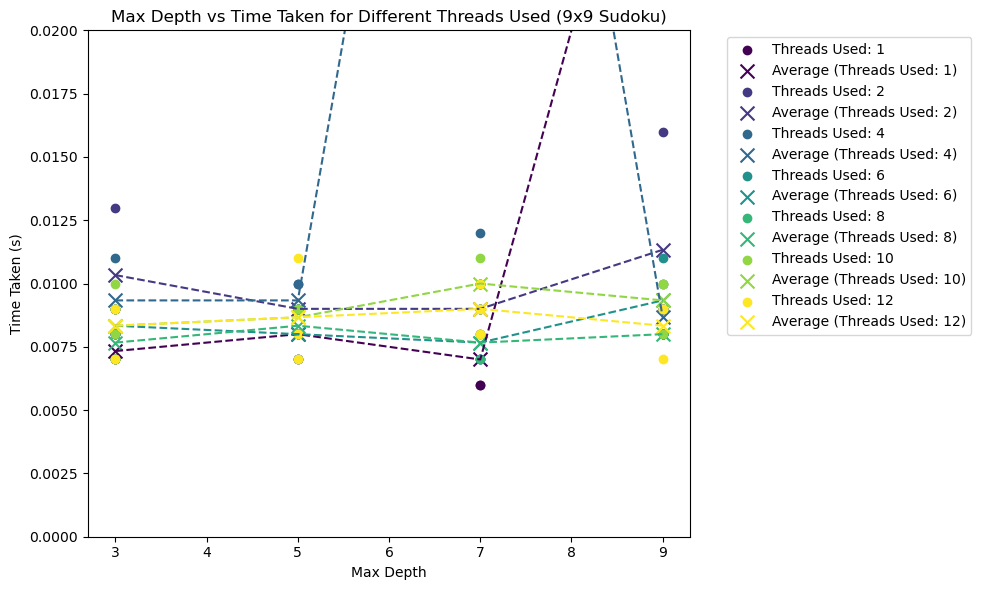
\includegraphics[width=\textwidth]{9x9_var_depth.png}
        \caption{Execution time for 9x9 Sudoku puzzles with variable depth.}
    \end{subfigure}
    \hfill
    \begin{subfigure}[b]{0.45\textwidth}
        \centering
        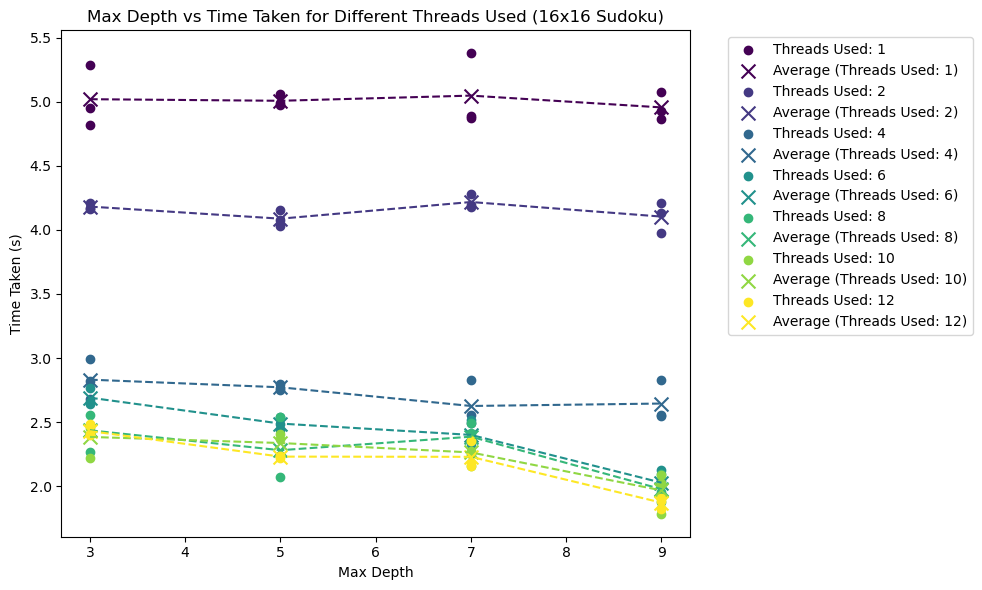
\includegraphics[width=\textwidth]{16x16_var_depth.png}
        \caption{Execution time for 16x16 Sudoku puzzles with variable depth.}
    \end{subfigure}
    \caption{Comparison of execution times for variable depth Sudoku puzzles.}
\end{figure}

For variable-depth experiments, performance trends are similarly unclear. The 9x9 Sudoku puzzles show minor gains with increasing thread counts at specific depths but reveal diminishing returns at higher depths. The 16x16 puzzles demonstrate significant variability, with some thread configurations performing worse as depth increases. These results highlight challenges in balancing task granularity and overhead when managing parallel recursion, emphasizing the need for better load-balancing strategies to maximize thread utilization effectively.

\section{Design Choices}

\begin{enumerate}
    \item \textbf{Parallelization with OpenMP:} The algorithm uses OpenMP to parallelize the Sudoku solving process. More specifically using the tasks directive.
    % \item \textbf{Recursive Backtracking:} The core of the algorithm is a recursive backtracking approach.
    \item \textbf{Depth Limitation:} To control the granularity of parallel tasks and avoid excessive task creation, the algorithm limits the depth of parallel recursion using the depth and max\_depth parameters.
    \item \textbf{Board Copying:} To avoid shared state issues between parallel tasks, the algorithm creates a copy of the Sudoku board for each task.
    \item \textbf{CSV Logging:} The algorithm logs the performance data to a CSV file.
\end{enumerate}

\section{Conclusions}

% The results of the experiments suggest it is not clear that increasing the number of threads consistently leads to performance improvements in the parallel Sudoku solver using a backtracking algorithm. The fixed-depth experiments show limited gains with more threads, while the variable-depth experiments exhibit significant variability in performance. The challenges in balancing task granularity, load distribution, and overhead management highlight the need for more sophisticated parallelization strategies to maximize thread utilization effectively. 

\end{document}
